\documentclass{book}

\title{Quantum Computing and Communication}
\newcommand{\booksubtitle}{A Textbook for Computer Science and Engineering Students}
\newcommand{\booklicense}{Creative Commons Zero 1.0 Universal}

\author{Yuan John Jiang}
% Author subtitle could be a university or a geographical location, for example
\newcommand{\authorsubtitle}{City, Country}

% Create convenient commands \booktitle and \bookauthor
\makeatletter
\newcommand{\booktitle}{\@title}
\newcommand{\bookauthor}{\@author}
\makeatother

% This utf8 declaration is not needed for versions of latex > 2018 but may
% be helpful for older software. Eventually it may not be worth keeping.
\usepackage[utf8]{inputenc}  
\usepackage{fix-cm}  % this package allows large \fontsize
\usepackage{tikz}    % this is for graphics. e.g. rectangle on title page
\usepackage{graphicx}
\usepackage{svg}
\usepackage{amsmath} % Used by equations

% The following dimensions specify 4.75" X 7.5" content on 6 3/8" by 9 1/4"
% paper. The paper width and height can be tweaked as required and the content
% should size to fit within the margins accordingly.
%
% The (inside) bindingoffset should be larger for books with more pages. Some
% standard recommended sizes are .375in minimum up to 1in for 600+ page books.
% Sizes .75in and .875in are also recommended roughly at 150 and 400 pages.
\usepackage[bindingoffset=0.625in,
            left=.5in, right=.5in,
            top=.8125in, bottom=.9375in,
            paperwidth=6.375in, paperheight=9.25in]{geometry}
% Here is an alternative geometry for reading on letter size paper:
% \usepackage[margin=.75in, paperwidth=8.5in, paperheight=11in]{geometry}

\renewcommand{\contentsname}{Table of Contents} % default is {Contents}
\usepackage{makeidx}
\makeindex % Initialize an index so we can add entries with \index

% The next few commands are for creating fake content to fill out the template.
% You should delete this (e.g.  everything up to, but not including,
% \begin{document}) after you insert your own content.
% Example content from Einstein's Meaning of Relativity.
% Public domain book: http://www.gutenberg.org/ebooks/36276

% Content Starts Here
\begin{document}
\frontmatter

% No page numbers on the Frontispiece page
% \thispagestyle{empty}


% ---- Title Page ----
% current geometry will be restored after title page
\newgeometry{top=1.75in,bottom=.5in}
\begin{titlepage}
\begin{flushleft}

% Title
\textbf{\fontfamily{qcs}\fontsize{38}{50}\selectfont Quantum Computing and\\ Communication}

% Draw a line 4pt high
\par\noindent\rule{\textwidth}{4pt}\\

% Shaded box from left to right with Subtitle
% The text node is midway (centered).
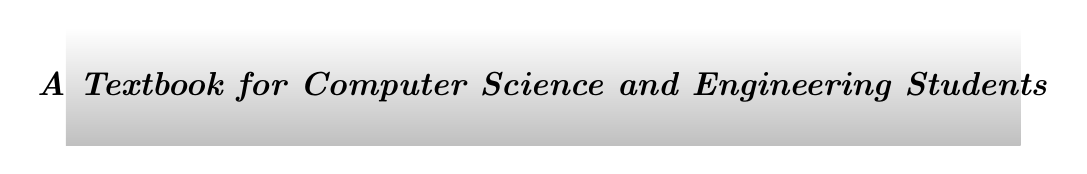
\begin{tikzpicture}
\shade[bottom color=lightgray,top color=white]
    (0,0) rectangle (\textwidth, 1.5)
    node[midway] {\textbf{\large \textit{\booksubtitle}}};
\end{tikzpicture}

% Edition Number
\begin{flushright}
\Large First Edition
\end{flushright}

\vspace{\fill}

% Author and Location
\textbf{\large \bookauthor}\\[3.5pt]
\textbf{\large \textit{\authorsubtitle}}

\vspace{\fill}

% Self Publishing Logo. Free to use: CC0 license.
% The source file is book.svg. If you change the svg, you must then convert
% it to pdf. There are many online and offline tools available to do that.
\begin{center}
%\includegraphics{booksvg.pdf}\\[4pt]
\fontfamily{lmtt}\small{Self Publishers Worldwide\\
}
\end{center}

\end{flushleft}
\end{titlepage}
\restoregeometry
% ---- End of Title Page ----

% Do not show page numbers on colophon page
\thispagestyle{empty}

\begin{flushleft}
\vspace*{\fill}
This book was typeset using \LaTeX{} software.\\
\vspace{\fill}
Copyright \textcopyright{} \the\year{}  \bookauthor\\
License: \booklicense
\end{flushleft}

% A title page resets the page # to 1, but the second title page
% was actually page 3. So add two to page counter.
\addtocounter{page}{2}

% The asterisk excludes chapter from the table of contents.
\chapter*{Preface}
Quantum computing and communication are hot topics. There are software development kits (SDKs), such as IBM Qiskit and Google Cirq, for programmers to develop quantum computer software. But there are no books on data structures and algorithms for computer science students. Similarly, there are no books on signaling and modulation for engineering students. This book is to bridge the gaps between quantum physics and engineering so that computer sciences and engineering students can use their knowledge to implement quantum algorithms and protocols or even develop them.

The difficulty of quantum physics lies in the wave behavior of particles. But that's the job of the physicists, and computer science and engineering students do not need to know. This book leaves out the details of the waves by labelling them with symbols e.g. "0" and "1". The symbols are what computer science and engineering students know how to work with. They are what data structure and algorithms in the computer science deal with, and what Shannon information theory apply to. There's absolutely no need to von Neumann entropy, which serves no purpose other than confusing non-physics majored.

How to use wave characteristics to represent information belongs to special subject of modulation. That is what  the communication engineering students know best. The book starts with how modulation works in qubits.

% Three-level Table of Contents
\setcounter{tocdepth}{3}
\tableofcontents

\mainmatter

\chapter{Introduction}
The advantage of quantum computing lies in the possibility of parallel computing. The use of quantum communication has been in key distribution. The secrecy of quantum key exchange lies in the uncertainty of quantum measurement. If these statements are too abstract, read on.

\section{The maze problems}
Maze problems are hard because there are too many paths to explore from the entrance to the exit. Computer scientists have long known parallel computing is the way to speed up solution finding of such problems.

\begin{figure}[ht]
\includegraphics[width=6cm]{maze.png}
\caption{Maze}
\label{Maze}
\end{figure}

People have always looked up to physicists to find ways to realize the solutions. Indeed, a physicist like me would suggest the following experiment to realize parallel computing: run water into the entrance and observe what's coming out of the exit. If we see water out of the exit, we know the maze problem has at least one solution. Of course, this is not the ultimate answer, which is to find all the good paths, we need. But at least it is the first useful step toward the ultimate solution.

The next step we may take is to ask the question: how many good paths are there. I would propose refining the experiment this way: run several water drops into the entrance and see how many drops will come out. Here, we run into the challenge of how to achieve the precision we need: if one drop comes out of the exit, how do we know whether there is only one good path or there are two drops from two paths arriving the exit at the same time. It would be ideal if we know what the smallest drop of water is like so that we can distinguish one drop from a combined two drops.

\section{The quantum power}
Playing with water tricks is exactly the idea behind quantum computers. Quantum physics tells us all matters are waves and have the smallest drops when measured the right way. A wave, like water, can spread and propagate through all possible paths and give us the power of parallel computing. The drop-like behavior (the so-called particle behavior by physicists) gives us the needed precision. We can also use the drop-like behavior in communication to assure that a communication channel is not tapped for eavesdropping because, if a bit carried by a smallest drop the carrier waves is tapped, it is lost as a whole. For this reason, quantum communication is the promise for ultimate secure communication.

\subsection{Waves}
Waves are not strangers to us. We use electromagnetic waves every day. We get Wi-Fi or cellphone signals even when we move around, in a house or on the streets, because the waves can spread and explore unlimited paths to reach us. So, we are already benefiting from the power of parallel exploration of waves.

For communication, we need waves that spread and propagate. They are propagating waves. Beside radio frequency waves propagating in free space, another type of propagating waves are used in optical communications. They are lights propagating in one dimension along the axis-es of the optical fibers. Because the waves are confined in the other two-dimensions and don't spread, we have minimal signal loss at the receiving ends.

We can also confine electromagnetic waves in three dimensions. Microwave ovens are examples. When confined this way, the waves do not propagate anywhere and are called standing waves. If no energy loss, a standing wave stays in the confinement forever. So, standing waves are good for storing information. The vibrations of a guitar string are also standing waves. The two ends of the string and fixed and block the vibration from propagating beyond the ends. When we pluck a string in a guitar, the vibration of the string does not go beyond its two ends. Superconductor qubits are built by standing waves of electrons as we will describe further below.

Another type of waves, which we may call trapped waves, are not confined but are trapped by forces extending to infinity. Electrons are trapped waves by the electric force of a nucleus' positive charges. The waves extend to infinity but are concentrated within a nanometer around the nucleus. Trapped waves are also good for storing information. Trapped-ion qubits are built by trapped electron waves.

By tradition, physicists use the bracket notations $|\phi>$ or $|\psi>$ to label waves and call them states.

\subsection{Particle behaviors and measurements}
Particles refer to things that are point like or of negligible sizes. Scientists believed electrons were particles when JJ Thomson discovered them in 1897. But when Ernest Rutherford discovered atomic nucleus 14 years later, people raised the question: why is the size of an atom much bigger than that of its nucleus? Why wouldn't the tiny negatively charged electrons fall into the positively charged nucleus and be combined into an atom close to the size of the nucleus -- if it were to happen, we would have not seen the world as we have.

We now know that electrons are not point like. So aren't the other so called particles, protons, neutrons etc. What we use to describe points, position or moment of time are not good quantities to describe them. Electric field and magnetic field strengths are still good quantities to measure. But when measuring quantities such as mass, energy, charge and what later discover in the 20th century such as "spin" and "flavor," physicists find their drop-like behavior. For example, the mass of electrons can only be multiple of $9.1x10^{-31}$ kg, and their charges can only be multiple of $1.6x10^{-19}$ Coulomb. And of course, the smallest drop is an electron. Physicists also know that lights have zero mass. But measuring their energy, physicists find their smallest drops and call them photons.

Physicists call the drop-like behavior particle behaviors. But the term "particle" misleads people to think of point-like objects. We try not to use the term in this book. The biggest implication of working with the smallest drop of a wave is that we only have one chance to measure the wave. After the measurement, the wave is in a changed form or course. Further, the impact of noise to a qubit leads to complete loss of information.

(Ignore - The waves we see or use everyday contain too many particles, and we only see the average effects of the waves and matters. If we pluck guitar string and hear the note E, which is different in our ears from that played on a violin. That is because the sound from each string on the respective instrument is composed by many harmonics, an octave apart from each other. The average or combined effects from the strings of different instruments is different. If our ears were sensitive enough to hear individual phonons -- the smallest drops of sound -- we would hear sound of pure harmonics.

Of course making such single particle, photon or phonon, generators or detectors has been the very challenge to physicists in their effort to make quantum computing and communication.)

\subsection{Information and modulations}
When we get our blood pressure measured in a doctor's office, the height of the mercury in a glass column represents the information of our blood pressur. The height of mercury in the column is what we actually measure and is what we use to represent the information of our blood pressure. Similarly, we use quatities such as the electric voltages in computer chips and circuits to represent the numbers we store or process. The methods to represent information in communication channels have a special name -- modulation. Radio broadcasts first used radio waves' amplitudes to represent the volume of one's voice. This is the so called amplitude modulation (AM). Later, frequency modulation (FM) was found less prone to the noise in the airways. That is why we now have both AM and FM on the panels of our radios.

Modulation -- how to represent information by electromagnetic waves for communications -- is one of the most important subjects studied for communication. That is because communication channels are prune to errors due to noises. Many names and acronyms in engineering books are in the subject in addition to AM and FM, e.g. phase modulation (PM) and quadrature amplitude modulation (QAM).

Not limited to communication, quantum computers are also prune to noises and errors because we work with the smallest drops of waves. How information is represented is also complicated as we will learn in the following sections. We will borrow the term "modulation" from communication textbooks to refer all the techniques for representing information as some physical characteristics. Understanding how modulation works in quantum computers and communication is the critical link for electrical engineering and computer science students to understand the quantum technologies. 

\subsection{Digital technology}
In theory, we can measure a wave's amplitude, frequency and phase precisely and use them to represent all real numbers. In really, our information transporting and processing devices have noises and errors. We are best to have the systems working with only integer numbers. Using integer numbers to represent information is what we call digital technology. In addition, using binary integers instead of decimals makes computer and communication components much simpler. And nowadays digital technology is almost the synonym of binary technology.

All electronic computers use digital technology if we ignore the history of the slide rules. Communication systems are slow to convert to digital technology. For a long time, communication was mostly about voice communication -- radio broadcast and telephones. For digital information, modulations such as AM, FM and PM often carry different names, e.g. amplitude-shift keying (ASK), frequency-shift keying (FSK) and phase-shift keying respectively (PSK).

Quadrature phase-shift keying (QPSK) uses one carrier wave to represent "0" and uses another, which is 90-degree phase shifted from the first, to represent "1". The second carrier wave is a quarter of wave phase shifted from the first is thus called the quadrature wave while the first is called the in-phase wave. The two waves are orthogonal from each other and thus are most immune to error -- best to distinguish one from another -- in the presence of noise.

Like QPSK, all qubits use two waves orthogonal to each other to represent "0" and "1" respectively. However, the orthogonality of the waves is not due to their phase difference but the result of their orthogonal polarizations or spatial concentrations. Another difference, QPSK can use additional carrier waves, $N$-degree phase shifted from the first, to represent more integers and thus more information. In electrical engineering textbooks, the design of QPSK is usually illustrated by as shown in Fig. \ref{8QPSK} is a constellation diagram of 8-QPSK, which uses 8 carrier waves with respective 0, 45, 90, 135, 180, 215, 270 and 315 degree phase shifts to represent 8 integers "0", "1", "2", ..., "7" (their binary symbols are 000, 001, 010, ..., 111).

\subsection{Qubits and modulations}
A quantum bit (qubit) is the fundamental quantum computer component to store one bit of information. The quantum communication unit for transporting one bit of information is also called a qubit. The way that the information is represented in a qubit is very much like how quadrature phase-shift keying (QPSK) works. QPSK uses one carrier wave to represent "0" and uses another carrier wave, which is 90-degree phase shifted from the first, to represent "1". The second carrier wave is a quarter of wave phase shifted from the first is thus called the quadrature wave. The two waves are orthogonal from each other and thus are most immune to error -- best to distinguish one from another -- in the presence of noise.

Like QPSK, all qubits use two waves orthogonal to each other to represent "0" and "1" respectively. However, the orthogonality of the waves is not due to their phase difference but the result of their orthogonal polarizations or spatial concentrations. Another difference, QPSK can use additional carrier waves, $N$-degree phase shifted from the first, to represent more integers and thus more information. In electrical engineering textbooks, the design of QPSK is usually illustrated by as shown in Fig. \ref{8QPSK} is a constellation diagram of 8-QPSK, which uses 8 carrier waves with respective 0, 45, 90, 135, 180, 215, 270 and 315 degree phase shifts to represent 8 integers "0", "1", "2", ..., "7" (their binary symbols are 000, 001, 010, ..., 111).
\begin{figure}[ht]
\includegraphics[width=6cm]{4qpsk.jpg}
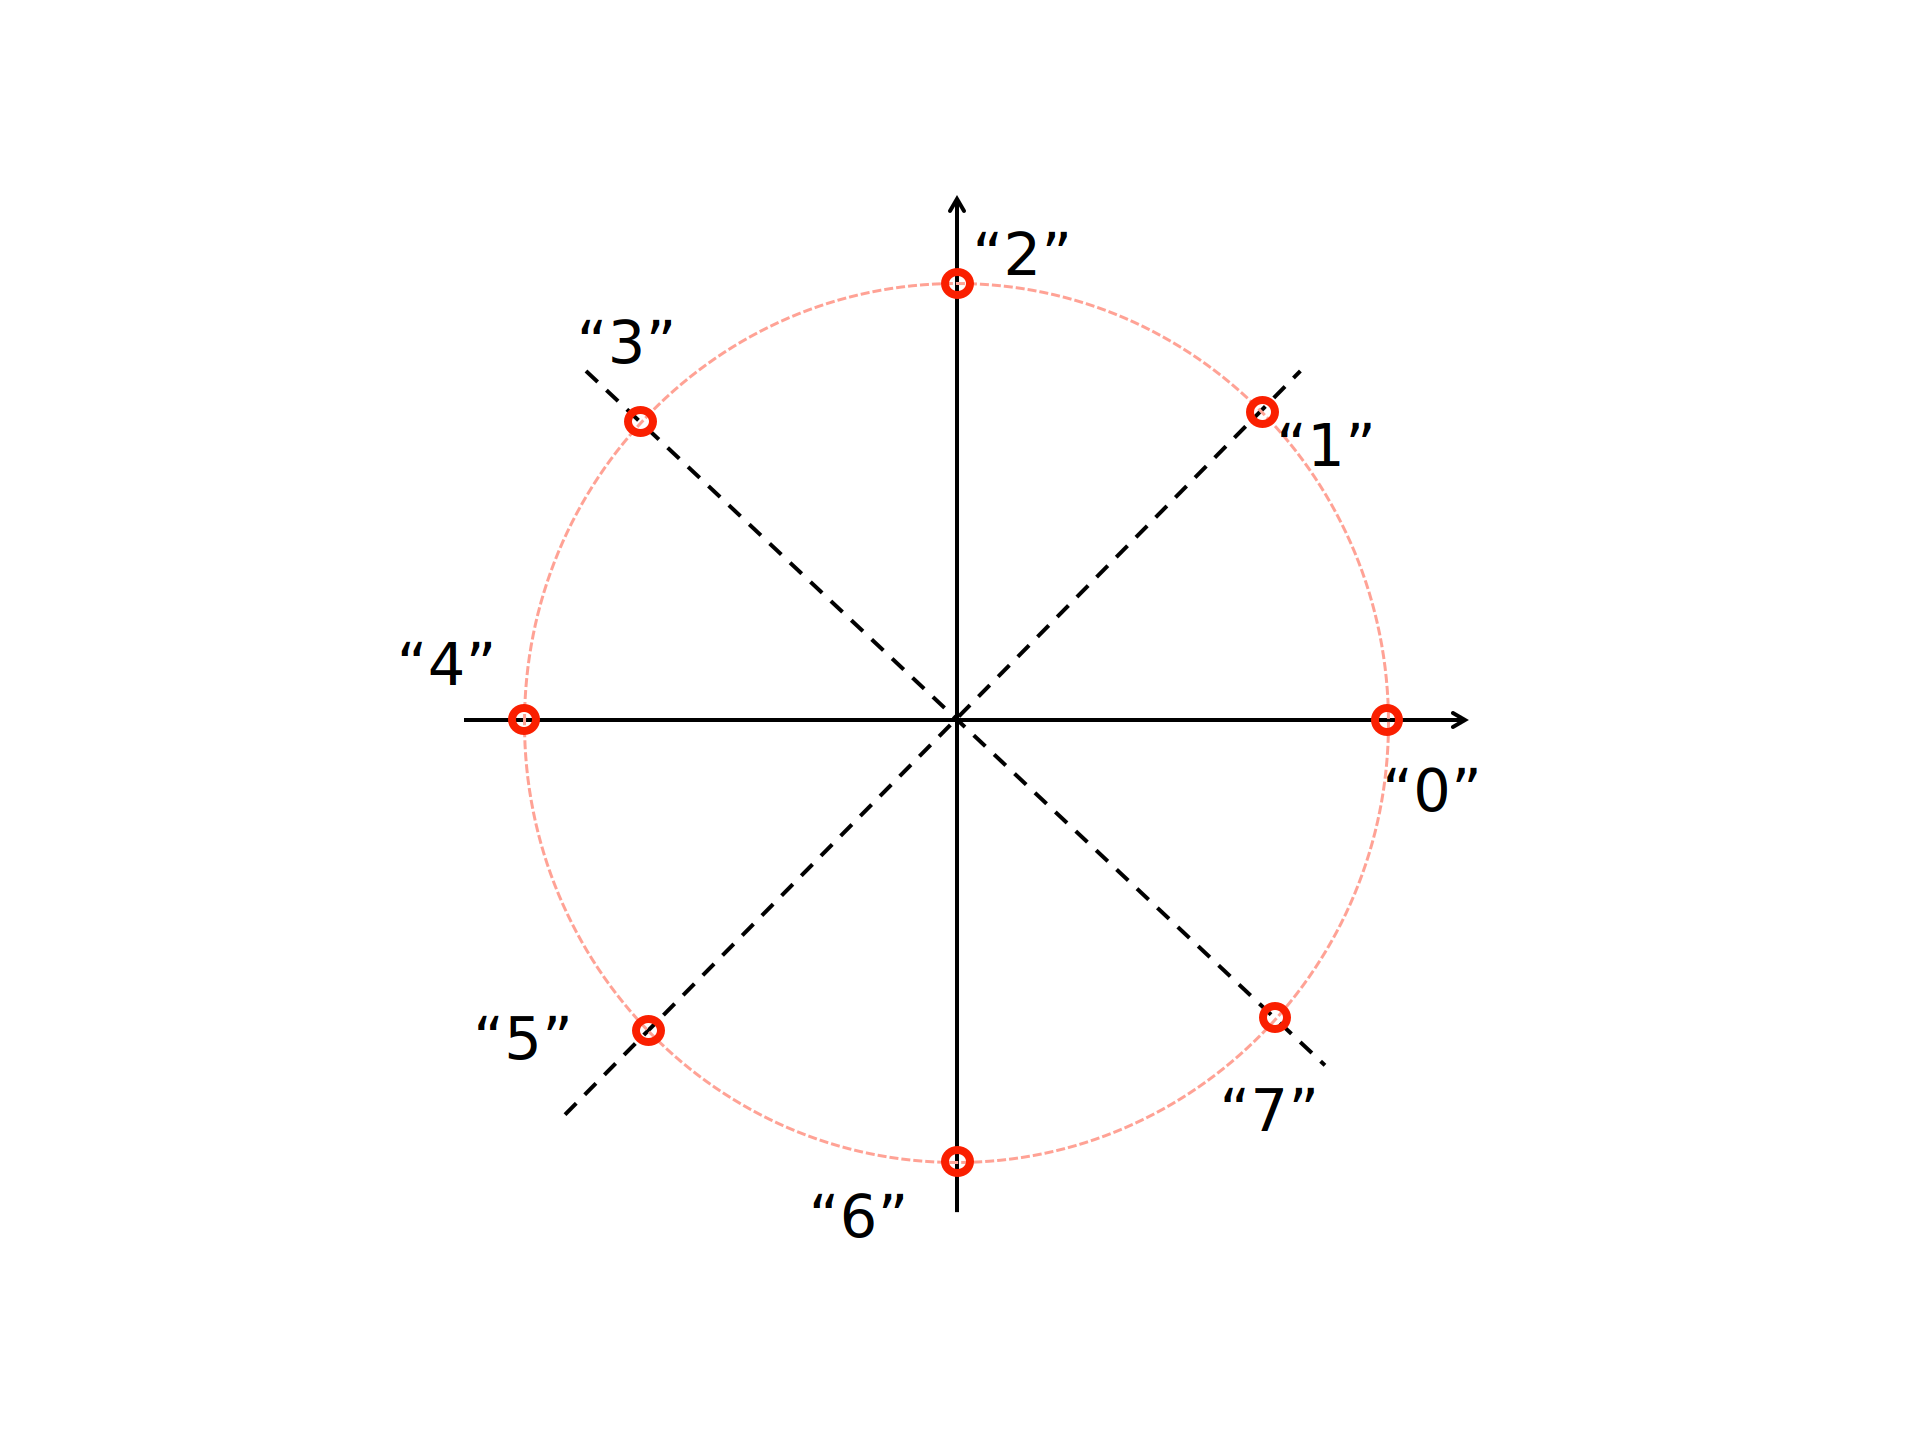
\includegraphics[width=6cm]{8qpsk.jpg}
\caption{Constellation diagrams of QPSK (left) and 8QPSK (right)}
\label{8QPSK}
\end{figure}
The waves that have 45, 135, 215 and 315 degree phase shifts can be viewed as combinations of the first wave and the quadrature. In quantum physics, such a composed wave is called a superposition state.

In qubits, we also use the 45 and 315 degree phase shifted waves, which are call the Bell states by physicists. But they are not used to represent more integers or information. In a computing qubit, we have one drop of the wave in both the "0" and "1" waves and achieve parallel exploration. For communication, a qubit in such a state obscures its true value to the eavesdropper. 
\begin{figure}[ht]
\includegraphics[width=6cm]{qqpsk.jpg}
\caption{Constenlation diagram of quantum phase shift keying}
\label{qQPSK}
\end{figure}

\subsubsection{Superconductor qubits}
A superconductor transmon qubit is similar to the string of a guitar and uses the first two standing waves, which resonate at the first and second harmonic frequencies respectively, to represent the integers of "0" and "1". Such a qubit is constructed by two superconductors separated by a layer of insulator. The insulator is thin enough for electrons to move ("tunnel") back and forth from one superconductor to another without loss of energy. But traveling through the insulator leads to delays (phase delays) of the electrons. The back-and-forth movement (vibration) of the electrons between the two superconductors resonate as standing waves at periods fractions of the delay. typically, the first fundamental frequency and the first harmonic are used to represent "0" and "1".
\begin{figure}[ht]
\includegraphics[width=6cm]{supercQubit.jpg}
\caption{Superconductor qubit}
\label{Superconductor}
\end{figure}

\begin{figure}[ht]
\includegraphics[width=6cm]{overtones.png}
\caption{The vibration of a string is a superposition of standing waves with wavelengths fractions of the string length.}
\label{Overtones}
\end{figure}

\subsubsection{Trapped ion qubits}

\subsubsection{Free space optical qubits}
Lights are propagating waves and obviously are suited for communications. The two waves used in such a qubit typically have the same frequency but different polarization's, orthogonal to each other.

\subsubsection{Optical waveguide qubits}
Another type of qubits uses lights -- traveling waves -- in waveguides. "0" is represented as light appearing in waveguide A while being absent in B; and "1" is represented as light appearing in waveguide B while being absent in A.
\begin{figure}[ht]
\includegraphics[width=6cm]{wguideQubit.png}
\caption{Waveguide qubit}
\label{Waveguide}
\end{figure}

\subsection{Bloch sphere}
(Ignore - If we consider the relative amplitude $A$ and phase $\phi$ of the two waves in a qubit, they can represent all the real number pairs in the rectangle ${ A \in [0,1], phi \in [0,2\pi) }$. Physicists like to represent the relative amplitude as $cos\theta$, and therefore, the $(\theta, \phi)$ pair can represent all the real number pairs in the rectangle ${[0,\pi],  [0,2\pi)}$. This rectangle can also be represented as a Bloch sphere.

\begin{figure}[ht]
\includegraphics[width=6cm]{blochSphere.png}
\caption{Bloch sphere}
\label{Bloch}
\end{figure}

If we measure waves in any than other way space or time, we find their smallest "drops" -- the particle nature of matter. Quantum physics started a hundred years ago when Einstein first proposed that electromagnetic waves, when measured in their energy, have the smallest drops called photons.

When measuring in electric charge, physicists discovered the smallest drops first and call them electrons before they realized their wave nature.

Measurement is the very thing that the quantum world is different from the classical world. In the quantum world, with an article, you only have one chance to measure it.)

\chapter{Quantum communication}
\section{BB84}
The key distribution protocol proposed by Charles Bennett and Gilles Brassard in 1984 is naturally called BB84. It is a rather boring protocol. It uses the fact that the key transmitting media are the smallest drops of waves and any eavesdropping can be detected. It uses two communication channels, one is an open and untrusted quantum channel, the other is an open but trusted classical channel.

The protocol works this way: Alice has a series of bits -- the secret key -- to transmit to Bob. Alice prepares another series random bits of equal length. Alice pairs one bit from each series into a number, 0, 1, 2, or 3, which are respectively 00, 01, 10 or 11 in binary, and send the number modulated according to Fig. \ref{qQPSK}. Bob has another random bits prepared. 

\section{Teleportation}
Alice has a qbit with information S and shares a pair of qbits with Bob. The pair is one of the 4 known eigenstates and has information 2. The total input information is therefore S+2. At the output, Alice measures the first 2 qbits against the same 4 eigenstates and tells Bob the result, which has information 2. If no information is lost, the information in the 3 qbit should be S.

\section{QSDC}

\chapter{Quantum computing}
\section{Data structures and quantum gates}
\subsection{Single qubits and Hadamaq gates}
\subsection{Entangled qubits and control gates}
\section{Deutsche algorithm}
\chapter{Bibliography}
\chapter{General Tendencies}

\backmatter
\addcontentsline{toc}{chapter}{Index}
\printindex
\end{document}